\documentclass[conference]{IEEEtran}
\usepackage[main=portuguese,provide=*]{babel}
\usepackage{cite}
\usepackage{amsmath,amssymb,amsfonts}
\usepackage{graphicx}
\usepackage{textcomp}
\usepackage{xcolor}
\usepackage[hidelinks]{hyperref}

\begin{document}

\title{Classificação de Flores Íris com k-NN: Análise Exploratória, PCA e Avaliação de Classificador}

\author{
    \IEEEauthorblockN{
        \begin{tabular}{c}
            Gustavo Gabriel Ripka \\
            GRR20203935
        \end{tabular}
        \qquad \qquad
        \begin{tabular}{c}
            Arthur Barreto Godoi \\
            GRR20224377
        \end{tabular}
    }
    \vspace{0.2cm}
    \IEEEauthorblockA{
        \textit{Departamento de Informática} \\
        \textit{Universidade Federal do Paraná -- UFPR}\\
        Curitiba, Brasil
    }
}

\maketitle

\begin{abstract}
Este trabalho realiza experimentos de classificação no dataset Íris, que contém comprimento e largura de sépalas e pétalas de três espécies de flores (\textit{Iris setosa}, \textit{Iris versicolor} e \textit{Iris virginica}), com 50 amostras cada. Inicialmente calculamos média, desvio padrão e moda de cada variável, no conjunto geral e por categoria, além da frequência de cada categoria. Em seguida analisamos a relação entre comprimento e largura da sépala e da pétala por categoria via regressão linear e correlação de Pearson, e examinamos a distribuição das categorias nas quatro dimensões. A Análise de Componentes Principais (PCA) mostrou que duas componentes concentram 95,8\% da variância total. Por fim, o dataset foi dividido em 80\% para treino e 20\% para teste, e um classificador k-NN foi ajustado por validação cruzada (melhor configuração: $k=5$, distância euclidiana, acurácia média de 96,7\% em validação cruzada), alcançando 93,3\% de acurácia no conjunto de teste, com erros concentrados na fronteira entre \textit{versicolor} e \textit{virginica}.
\end{abstract}

\begin{IEEEkeywords}
dataset Íris, análise exploratória, correlação, PCA, k-NN, validação cruzada.
\end{IEEEkeywords}

\section{Introdução}
Reconhecimento de padrões é uma tarefa central em visão computacional: dado um conjunto de medidas (atributos) de objetos, deseja-se atribuir a cada objeto uma categoria \cite{todt2026}. Um classificador supervisionado aprende essa correspondência a partir de exemplos rotulados, e sua avaliação honesta exige separar os dados usados para ajuste daqueles usados para teste \cite{todt2026knn}.

Neste trabalho usamos o dataset Íris \cite{fisher1936,uciiris}, um dos conjuntos de dados mais conhecidos da literatura, formado por 150 flores igualmente distribuídas em três categorias. Cada flor é descrita por quatro medidas em centímetros: comprimento da sépala (CS), largura da sépala (LS), comprimento da pétala (CP) e largura da pétala (LP). O objetivo é percorrer o ciclo completo de um experimento de classificação: estatística descritiva, análise de relações entre variáveis, visualização da distribuição das categorias, redução de dimensionalidade com PCA e, por fim, separação das classes com o classificador k-vizinhos-mais-próximos (k-NN) \cite{todt2026knn}.

O restante do relatório está organizado da seguinte forma: a Seção~\ref{sec:metodos} descreve materiais e métodos; a Seção~\ref{sec:descritiva} apresenta a estatística descritiva; a Seção~\ref{sec:relacoes} analisa as relações comprimento $\times$ largura; a Seção~\ref{sec:distribuicao} examina a distribuição nas quatro dimensões; a Seção~\ref{sec:pca} apresenta a PCA; a Seção~\ref{sec:knn} descreve os experimentos de classificação com k-NN; e a Seção~\ref{sec:conclusao} conclui.

\section{Materiais e Métodos}
\label{sec:metodos}
Os experimentos foram implementados em Python 3 com as bibliotecas NumPy, pandas, SciPy, Matplotlib e scikit-learn \cite{sklearn}. O dataset original do UCI Machine Learning Repository \cite{uciiris} foi usado na forma do arquivo \texttt{iris.data} (150 linhas, sem valores ausentes). Para reprodutibilidade, todas as operações aleatórias usaram semente fixa igual a 42.

A metodologia seguiu as etapas: (i) estatística descritiva geral e por categoria, com frequências; (ii) análise da relação comprimento $\times$ largura da sépala e da pétala por categoria, com regressão linear simples e coeficiente de correlação de Pearson $r$; (iii) matriz de dispersão das quatro variáveis para examinar a distribuição das categorias; (iv) PCA sobre dados padronizados (z-score); (v) divisão estratificada 80\%/20\% em treino/teste; e (vi) classificação com k-NN, com seleção de hiperparâmetros por validação cruzada em 5 partições (\textit{5-fold cross-validation}) apenas no conjunto de treino, seguida de avaliação única no conjunto de teste \cite{todt2026knn}.

\section{Estatística Descritiva}
\label{sec:descritiva}

A Tabela~\ref{tab:geral} resume média, desvio padrão e moda das quatro variáveis no conjunto geral (150 flores). As pétalas apresentam os maiores desvios padrão relativos (CP: 1,76\,cm; LP: 0,76\,cm), indicando alta variabilidade — reflexo direto das diferenças entre as espécies. As sépalas variam menos (CS: 0,83\,cm; LS: 0,43\,cm).

\begin{table}[htbp]
\caption{Estatística descritiva no conjunto geral ($n=150$). Valores em cm.}
\label{tab:geral}
\centering
\begin{tabular}{lccc}
\hline
Variável & Média & Desvio padrão & Moda \\
\hline
Comprimento sépala & 5,84 & 0,83 & 5,0 \\
Largura sépala & 3,05 & 0,43 & 3,0 \\
Comprimento pétala & 3,76 & 1,76 & 1,5 \\
Largura pétala & 1,20 & 0,76 & 0,2 \\
\hline
\end{tabular}
\end{table}

A Tabela~\ref{tab:classes} mostra as estatísticas por categoria. A frequência de cada categoria é idêntica: 50 flores (33,3\%) de cada espécie, ou seja, o dataset é perfeitamente balanceado.

Observa-se um padrão claro de separação em tamanho de pétala: \textit{setosa} tem pétalas pequenas (CP médio 1,46\,cm), \textit{versicolor} intermediárias (4,26\,cm) e \textit{virginica} grandes (5,55\,cm), com intervalos quase disjuntos. As sépalas separam menos: \textit{setosa} tem a maior largura média de sépala (3,42\,cm) apesar do menor comprimento (5,01\,cm), enquanto \textit{virginica} tem as maiores sépalas em comprimento (6,59\,cm).

\begin{table}[htbp]
\caption{Média $\pm$ desvio padrão por categoria ($n=50$ cada). Valores em cm.}
\label{tab:classes}
\centering
\begin{tabular}{lccc}
\hline
Variável & Setosa & Versicolor & Virginica \\
\hline
Compr. sépala & 5,01 $\pm$ 0,35 & 5,94 $\pm$ 0,52 & 6,59 $\pm$ 0,64 \\
Largura sépala & 3,42 $\pm$ 0,38 & 2,77 $\pm$ 0,31 & 2,97 $\pm$ 0,32 \\
Compr. pétala & 1,46 $\pm$ 0,17 & 4,26 $\pm$ 0,47 & 5,55 $\pm$ 0,55 \\
Largura pétala & 0,24 $\pm$ 0,11 & 1,33 $\pm$ 0,20 & 2,03 $\pm$ 0,28 \\
\hline
\end{tabular}
\end{table}

\section{Relação Comprimento $\times$ Largura}
\label{sec:relacoes}

\subsection{Sépalas}
A Fig.~\ref{fig:sepalas} mostra a dispersão comprimento $\times$ largura da sépala por categoria, com reta de regressão linear ajustada. As correlações de Pearson são moderadas e positivas nas três categorias: $r = 0{,}75$ para \textit{setosa} ($p < 0{,}001$), $r = 0{,}53$ para \textit{versicolor} ($p < 0{,}001$) e $r = 0{,}46$ para \textit{virginica} ($p < 0{,}001$). Ou seja, dentro de cada espécie, sépalas mais longas tendem a ser também mais largas, com a relação mais forte em \textit{setosa}. No plano sépala, porém, as categorias \textit{versicolor} e \textit{virginica} se sobrepõem fortemente — a variável sépala sozinha não separa bem essas duas espécies.

\begin{figure}[htbp]
\centerline{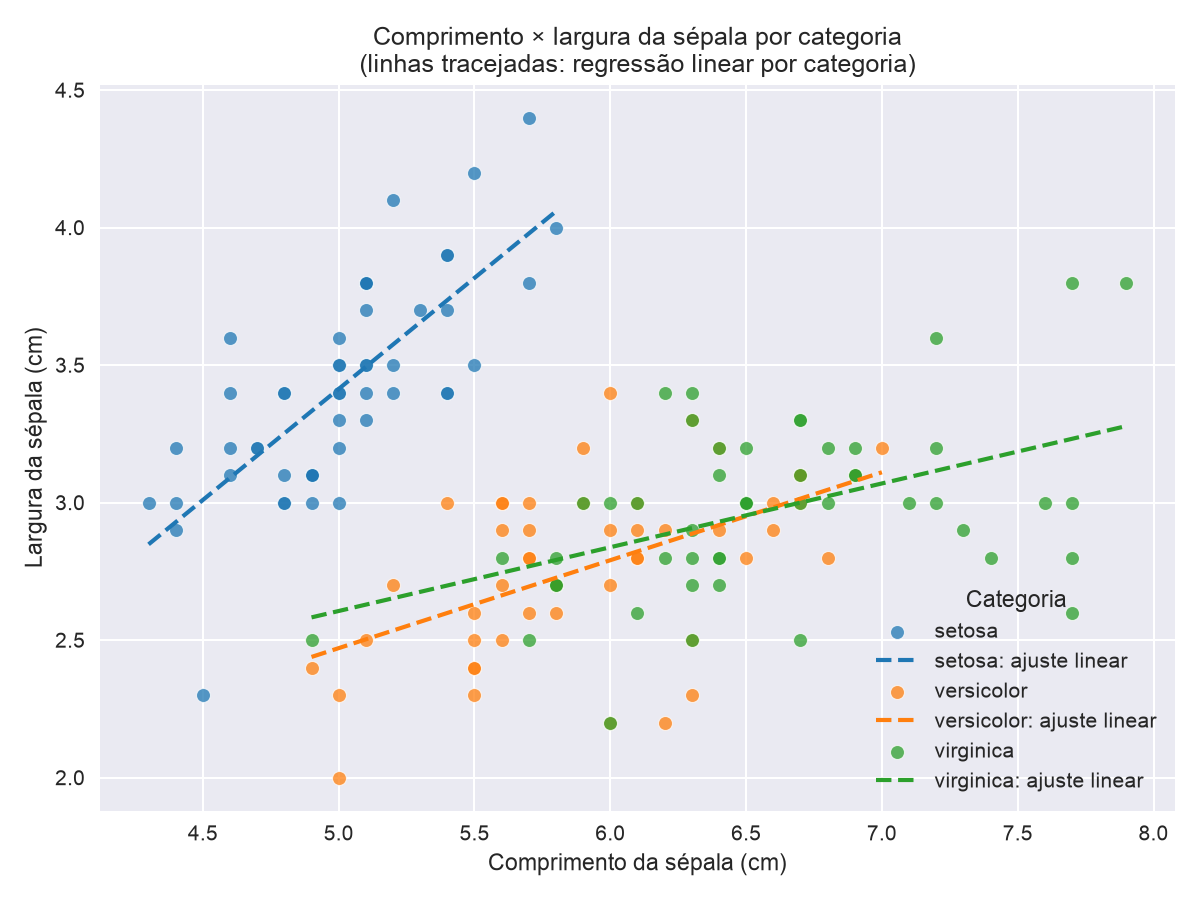
\includegraphics[width=\linewidth]{figs/sepalas_dispersao.png}}
\caption{Comprimento $\times$ largura da sépala por categoria, com retas de regressão linear.}
\label{fig:sepalas}
\end{figure}

\subsection{Pétalas}
A Fig.~\ref{fig:petalas} mostra o mesmo tipo de análise para as pétalas. As correlações são $r = 0{,}31$ para \textit{setosa} ($p = 0{,}031$), $r = 0{,}79$ para \textit{versicolor} ($p < 0{,}001$) e $r = 0{,}32$ para \textit{virginica} ($p = 0{,}023$). A relação linear é forte apenas em \textit{versicolor}; em \textit{setosa} e \textit{virginica} o tamanho da pétala varia pouco em largura, enfraquecendo a correlação. O ponto mais importante, porém, é a separação: no plano pétala, \textit{setosa} fica completamente isolada (pétalas curtas e estreitas), e a fronteira entre \textit{versicolor} e \textit{virginica}, embora exista, ainda apresenta sobreposição parcial.

\begin{figure}[htbp]
\centerline{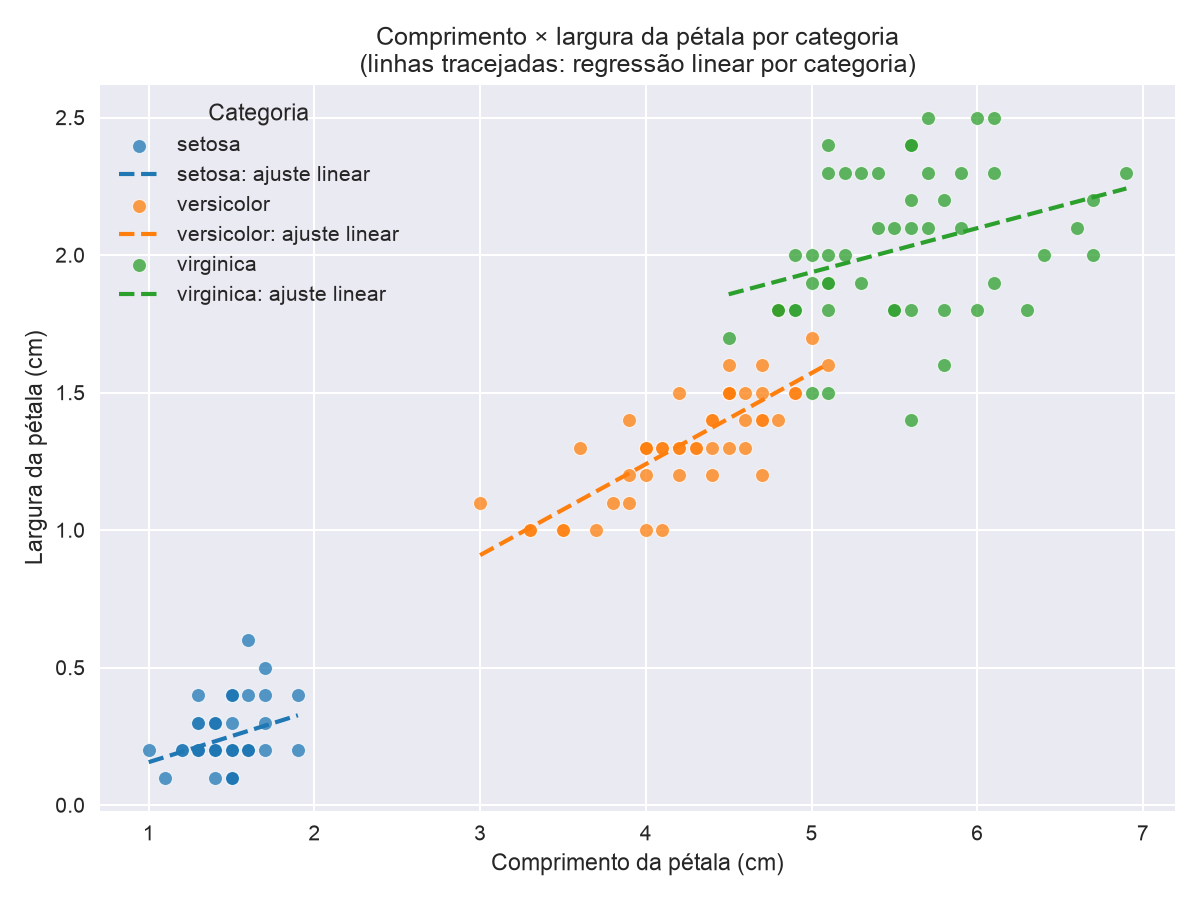
\includegraphics[width=\linewidth]{figs/petalas_dispersao.png}}
\caption{Comprimento $\times$ largura da pétala por categoria, com retas de regressão linear.}
\label{fig:petalas}
\end{figure}

\section{Distribuição nas Quatro Dimensões}
\label{sec:distribuicao}

A Fig.~\ref{fig:matriz} apresenta a matriz de dispersão das quatro variáveis, com histogramas na diagonal. A leitura por pares de variáveis confirma: (i) \textit{setosa} é linearmente separável das demais em praticamente qualquer par envolvendo pétalas; (ii) \textit{versicolor} e \textit{virginica} se misturam nos pares de sépalas e se separam parcialmente nos pares envolvendo comprimento de pétala, com melhor resultado quando CP e LP são combinadas. Os histogramas diagonais mostram ainda que as distribuições de CP e LP são claramente trimodais no conjunto geral — cada moda corresponde a uma espécie —, enquanto as variáveis de sépala têm distribuições unimodais sobrepostas.

\begin{figure*}[htbp]
\centerline{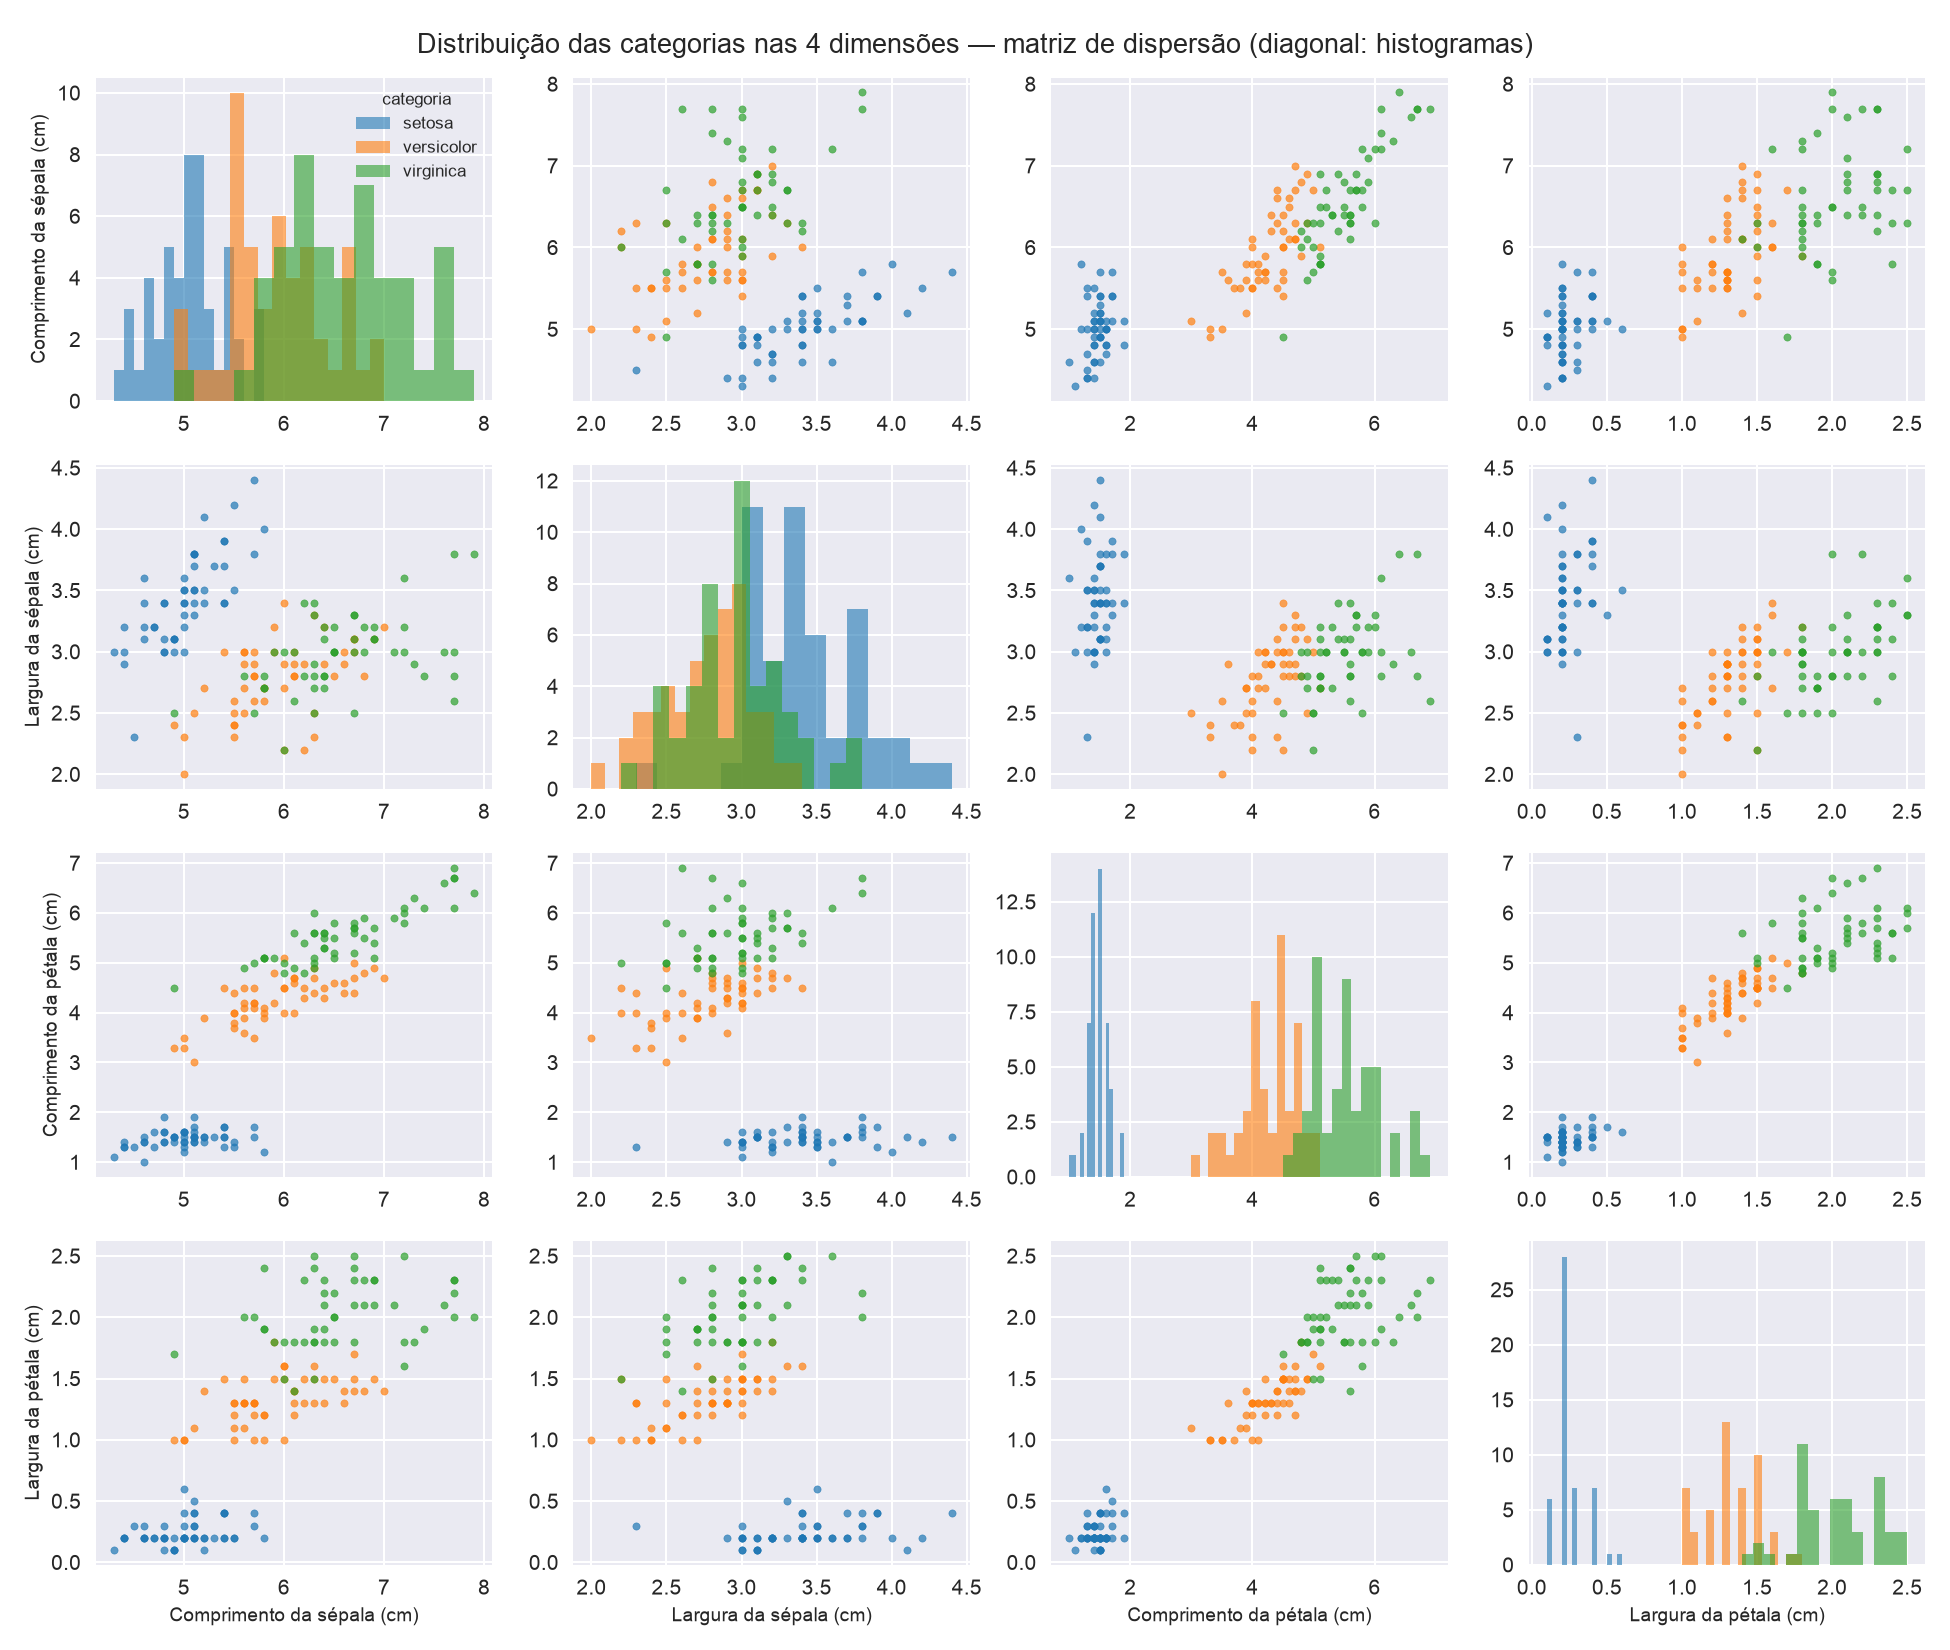
\includegraphics[width=0.9\textwidth]{figs/matriz_dispersao.png}}
\caption{Matriz de dispersão das quatro variáveis (cm) com histogramas na diagonal.}
\label{fig:matriz}
\end{figure*}

\section{Análise de Componentes Principais}
\label{sec:pca}

A PCA \cite{jolliffe2016} projeta os dados em direções ortogonais de máxima variância. Aplicamos a PCA sobre os dados padronizados (média 0, desvio 1), etapa recomendada quando as variáveis têm escalas ou variabilidades diferentes. Os resultados (Fig.~\ref{fig:pca}) mostram que a primeira componente principal (PC1) explica 72,8\% da variância e a segunda (PC2) 23,0\%, totalizando 95,8\% com apenas duas dimensões — as demais componentes contribuem com apenas 3,7\% (PC3) e 0,5\% (PC4).

Os pesos (\textit{loadings}) da PC1 são dominados pelas medidas de pétala (CP: 0,58; LP: 0,57) e pelo comprimento de sépala (0,52), com contribuição negativa pequena da largura de sépala ($-0$,26): PC1 é essencialmente um eixo de ``tamanho geral da flor'', com destaque para as pétalas. A PC2 é dominada pela largura de sépala (0,93), um eixo quase independente do primeiro.

Na projeção PC1 $\times$ PC2, \textit{setosa} forma um grupo isolado, e \textit{versicolor}/\textit{virginica} formam grupos adjacentes com pequena sobreposição — consistente com a análise por pares. O resultado é interessante do ponto de vista prático: as 4 medidas podem ser reduzidas a 2 componentes com perda mínima de informação (95,8\% da variância preservada), o que facilita visualização e pode reduzir custo de cálculo em classificadores por distância como o k-NN.

\begin{figure}[htbp]
\centerline{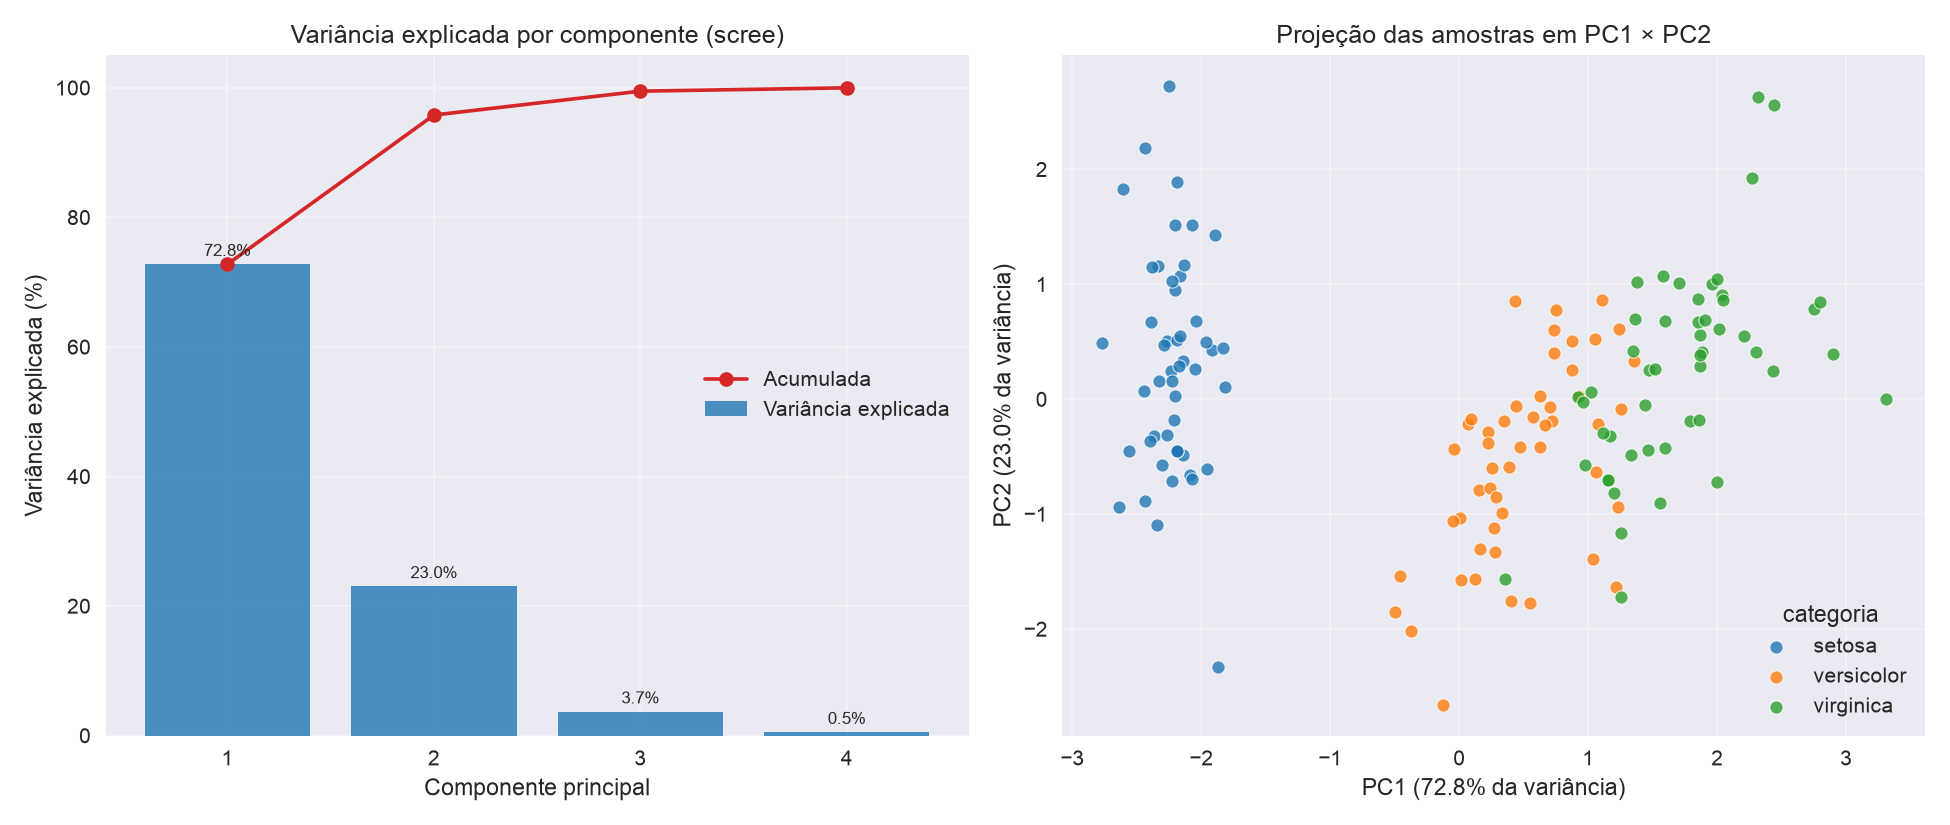
\includegraphics[width=\linewidth]{figs/pca.png}}
\caption{PCA sobre dados padronizados: variância explicada (esquerda) e projeção PC1 $\times$ PC2 (direita).}
\label{fig:pca}
\end{figure}

\section{Classificação com k-NN}
\label{sec:knn}

\subsection{Divisão treino/teste e metodologia}
O dataset foi dividido em 80\% para treino (120 amostras) e 20\% para teste (30 amostras), com amostragem estratificada: 40/40/40 por categoria no treino e 10/10/10 no teste, preservando o balanceamento original.

O classificador k-NN \cite{todt2026knn} não constrói um modelo explícito: ele memoriza os exemplos de treino e classifica uma nova amostra pela maioria entre os $k$ vizinhos mais próximos, segundo uma métrica de distância. Como o k-NN se baseia em distâncias, as variáveis foram padronizadas com \texttt{StandardScaler} ajustado apenas no treino, evitando que variáveis de escala maior dominem o cálculo \cite{todt2026knn}. Os hiperparâmetros $k \in \{1, 3, \dots, 21\}$ e a métrica (euclidiana ou Manhattan) foram selecionados por \textit{grid search} com validação cruzada de 5 partições no conjunto de treino.

\subsection{Seleção de hiperparâmetros}
A Fig.~\ref{fig:knn} mostra a acurácia média de validação cruzada em função de $k$ para as duas métricas. A melhor configuração foi $k=5$ com distância euclidiana (acurácia média de 96,7\% $\pm$ 3,1\%). O desempenho é estável em uma ampla faixa ($k$ entre 3 e 21 fica acima de 95\%), com degradação leve para $k$ grandes, e a métrica euclidiana foi consistentemente igual ou superior à Manhattan.

\begin{figure}[htbp]
\centerline{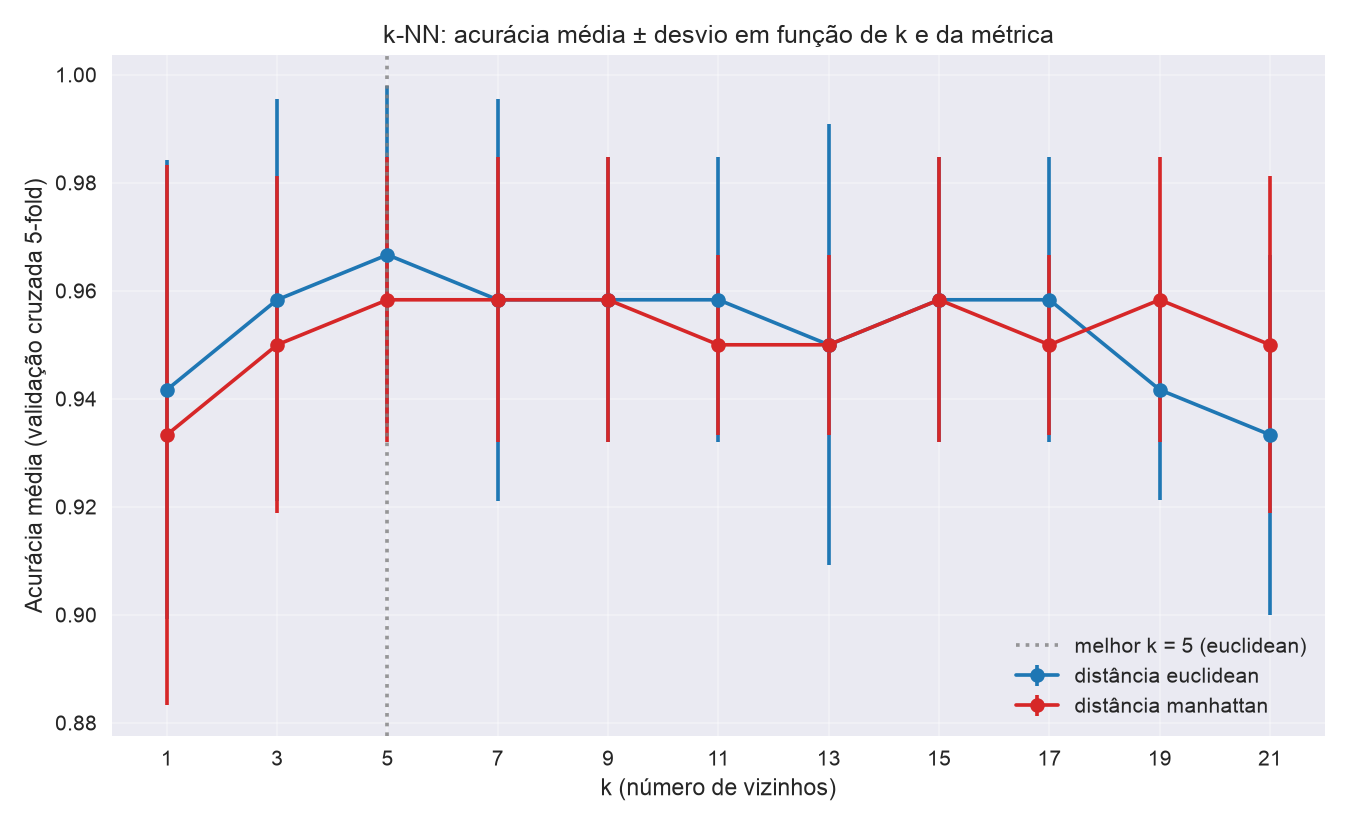
\includegraphics[width=\linewidth]{figs/knn_cv.png}}
\caption{Acurácia média (5-fold) no treino em função de $k$, para distâncias euclidiana e Manhattan.}
\label{fig:knn}
\end{figure}

\subsection{Resultados no teste}
Com $k=5$ e distância euclidiana, o modelo alcançou \textbf{acurácia de 93,3\%} (28 acertos em 30) no conjunto de teste. A Tabela~\ref{tab:relatorio} mostra o relatório de classificação por classe: \textit{setosa} é classificada perfeitamente (F1 = 1,00); os erros concentram-se na fronteira \textit{versicolor}--\textit{virginica}. A matriz de confusão (Fig.~\ref{fig:confusao}) confirma: as duas amostras erroneamente classificadas são \textit{virginica} previstas como \textit{versicolor} — exatamente a região de sobreposição identificada na análise exploratória e na PCA.

\begin{table}[htbp]
\caption{Relatório de classificação no conjunto de teste ($k=5$, euclidiana).}
\label{tab:relatorio}
\centering
\begin{tabular}{lcccc}
\hline
Classe & Precisão & Revocação & F1 & Suporte \\
\hline
Setosa & 1,00 & 1,00 & 1,00 & 10 \\
Versicolor & 0,83 & 1,00 & 0,91 & 10 \\
Virginica & 1,00 & 0,80 & 0,89 & 10 \\
\hline
Média macro & 0,94 & 0,93 & 0,93 & 30 \\
\hline
\end{tabular}
\end{table}

\begin{figure}[htbp]
\centerline{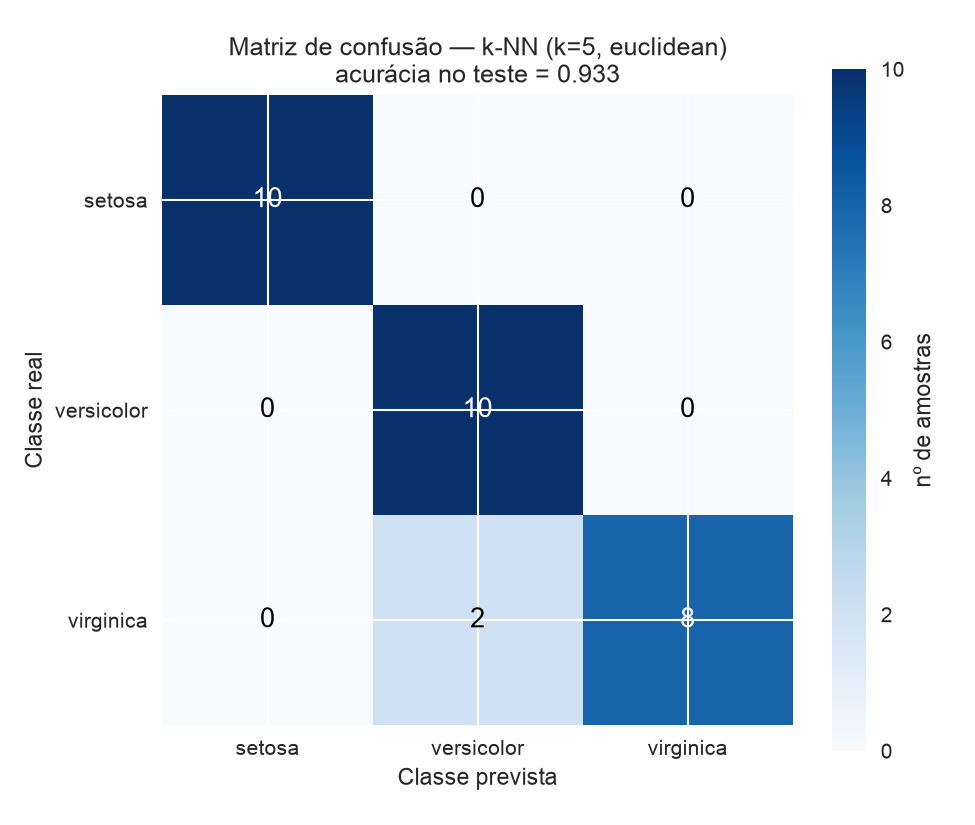
\includegraphics[width=\linewidth]{figs/matriz_confusao.png}}
\caption{Matriz de confusão no conjunto de teste (linhas: classe real; colunas: classe prevista).}
\label{fig:confusao}
\end{figure}

Vale registrar duas observações. Primeiro, $k=1$ (NN puro, com padronização) obteve 96,7\% neste teste particular; ainda assim mantivemos $k=5$, escolhido exclusivamente com dados de treino/validação — usar o resultado do teste para trocar de modelo caracterizaria vazamento de informação. Segundo, rodando sem padronização o k-NN acertou as 30 amostras (100\%). Isso não contradiz a recomendação do escalonamento \cite{todt2026knn}: no Íris as quatro variáveis têm escalas próximas (0,1--7,9\,cm), então a padronização pouco altera as distâncias, e a diferença observada decorre de sorte amostral num teste pequeno (30 amostras). Em domínios com escalas heterogêneas (e.g., intensidades de pixel 0--255 combinadas com outras medidas), a padronização é indispensável.

\section{Conclusão}
\label{sec:conclusao}
O ciclo completo de experimentos no dataset Íris mostrou que a estatística descritiva e a análise de relações entre variáveis já revelam a estrutura do problema: pétalas separam bem as espécies (padrão trimodal, \textit{setosa} isolada), enquanto sépalas separam pouco, e as correlações comprimento $\times$ largura variam de fracas a fortes conforme a espécie e o órgão da flor. A PCA condensou 95,8\% da variância em duas componentes, cuja projeção reproduz a geometria das classes vista nos pares de variáveis.

O classificador k-NN com padronização, $k=5$ e distância euclidiana — selecionado por validação cruzada — alcançou 93,3\% de acurácia no teste, com erros restritos à fronteira \textit{versicolor}--\textit{virginica}, coerentes com a sobreposição observada na análise exploratória. Os resultados ilustram na prática conceitos das aulas: memorização vs.\ generalização, papel da métrica de distância e do escalonamento, seleção de hiperparâmetros por validação cruzada e avaliação honesta em conjunto de teste separado. Como trabalho futuro, seria natural comparar o k-NN com outros classificadores (e.g., SVM, árvores de decisão) e usar as duas primeiras componentes principais como entrada do classificador.

\begin{thebibliography}{00}
\bibitem{todt2026} E. Todt, ``Computer Vision and Perception: Recognition,'' Aula 1, Departamento de Informática, UFPR, 2026.
\bibitem{todt2026knn} E. Todt, ``Computer Vision and Perception: Classification -- kNN,'' Aula 2, Departamento de Informática, UFPR, 2026.
\bibitem{fisher1936} R. A. Fisher, ``The use of multiple measurements in taxonomic problems,'' \textit{Annals of Eugenics}, vol. 7, no. 2, pp. 179--188, 1936.
\bibitem{uciiris} ``Iris Data Set,'' UCI Machine Learning Repository. [Online]. Available: \url{https://archive.ics.uci.edu/ml/datasets/iris}
\bibitem{jolliffe2016} I. T. Jolliffe e J. Cadima, ``Principal component analysis: a review and recent developments,'' \textit{Philosophical Transactions of the Royal Society A}, vol. 374, 2016.
\bibitem{sklearn} F. Pedregosa \textit{et al.}, ``Scikit-learn: Machine Learning in Python,'' \textit{Journal of Machine Learning Research}, vol. 12, pp. 2825--2830, 2011.
\end{thebibliography}

\end{document}
